%%%%%%%%%%%%%%%%%%%%%%%%%%%%%%%%%%%%%%%%%
% University/School Laboratory Report
% LaTeX Template
% Version 3.1 (25/3/14)
%
% This template has been downloaded from:
% http://www.LaTeXTemplates.com
%
% Original author:
% Linux and Unix Users Group at Virginia Tech Wiki 
% (https://vtluug.org/wiki/Example_LaTeX_chem_lab_report)
%
% License:
% CC BY-NC-SA 3.0 (http://creativecommons.org/licenses/by-nc-sa/3.0/)
%
%%%%%%%%%%%%%%%%%%%%%%%%%%%%%%%%%%%%%%%%%

%----------------------------------------------------------------------------------------
%	PACKAGES AND DOCUMENT CONFIGURATIONS
%----------------------------------------------------------------------------------------

\documentclass{article}

\usepackage{graphicx} % Required for the inclusion of images
%\usepackage{natbib} % Required to change bibliography style to APA
\usepackage{amsmath} % Required for some math elements 
\usepackage{geometry}
\usepackage{float}
\usepackage{url}
%\usepackage{biblatex}

\geometry {a4paper, left = 30mm}
\renewcommand{\baselinestretch}{1.5}
\setlength{\parskip}{1em}
\setlength\parindent{0pt} % Removes all indentation from paragraphs

\renewcommand{\labelenumi}{\alph{enumi}.} % Make numbering in the enumerate environment by letter rather than number (e.g. section 6)

%\usepackage{times} % Uncomment to use the Times New Roman font

%----------------------------------------------------------------------------------------
%	DOCUMENT INFORMATION
%----------------------------------------------------------------------------------------

\title{COSC450: Procedural City Generation} % Title

\author{Joshua La Pine} % Author name

\begin{document}

\maketitle % Insert the title, author and date

\begin{center}
Dept. of Computer Science \\
Otago University \\

\end{center}
\newpage
% If you wish to include an abstract, uncomment the lines below
% \begin{abstract}
% Abstract text
% \end{abstract}

%----------------------------------------------------------------------------------------
%	SECTION 1
%----------------------------------------------------------------------------------------

\section{Planning and Difficulties}

When deciding on how best to approach this assignment there were several key ideas that came to mind. First and foremost was my desire to render a city with a layout beyond a standard, evenly spaced grid. Initially my plan was to generate a series of 'city blocks', each block a plane with three, four, or five vertices. The vertices of these blocks would be placed in a vaguely grid based way but with their specific locations determined pseudo-randomly. A vertex's location was to be the product of it's appoximate location in the 'grid', the locations of surrounding vertices, and the number of vertices comprising that particular block. I was about 200 lines of python deep before I realised the complexity of what I had imagined. For example, if I wanted the edges of the city to be straight I had to program a case for each edge piece, that is a special case for the left, right, top, and bottom edges of the city, not to mention the corner pieces which would have required two straight edges. Then there is the issue of how to determine the placement of internal vertices. I had envisioned a city where a block with an angled edge would have a neighbour with an edge parallel to it, where blocks could be multiple different sizes and shapes and the surrounding blocks would be placed in such a way that the space was filled. I was forced to abandon this approach when I realised that this was too complex for the amount of time I had to complete the assignment. \par

Not wanting to give up on a non-grid based layout I came up with another idea. I would start with a plane and would then bisect that plane repeatedly into different meshes to create a collection of blocks. The plan was to bisect the original mesh into rows and then split each row into columns with the angle of the split and width of the block being randomised each time but with a bias towards straight lines and thin blocks. I had hoped that this would create a grid like pattern but one that was more interesting to look at. This turned out to be another dead end primarily due to the blender functions available. A bisection doesn't return a reference to the newly created mesh, it only puts the new mesh into the scene's object array. As I was unable to find out how it determined the index of the new mesh I had to abandon this idea as well.\par

So after four days of wasted effort I decided to create a typical grid based layout for my city. In order to make my city more complex I decided to create various block layouts and different kinds of buildings, as well as a function that determines the type of building to create based on distance from the centre of the city. 

\section{Implementation}

My city generation script begins by creating a grid of 'city blocks'. These blocks are simple squares with a depth and side length defined as a parameter at the top of the script. The number of rows and columns of the grid is similarly defined. Each of these blocks is defined by its vertices which are calculated in a loop and then used to create a mesh which is stored in an array for later referencing.\par

Once the city block grid has been generated, each block must be divided further into sub-blocks. For each city block, I get the global coordinates of it's top-left and bottom-right vertices. From these coordinates you have all the information you need to subdivide the block how you want. For my purposes I defined a set of possible sub-blocks and then created a list for every valid combination of sub-blocks, that is, every combination that would fit on a city block. There are eight possible sub-block combinations as can be seen below in Figure 1. A sub-block is defined as a list comprising the global x and y coordinates of its top-left and bottom-right corners. A sub-block has no pyhsical component like a city block, as it is simply used to define the area in which a building must be contained. \par

\begin{figure}[H]
\begin{center}
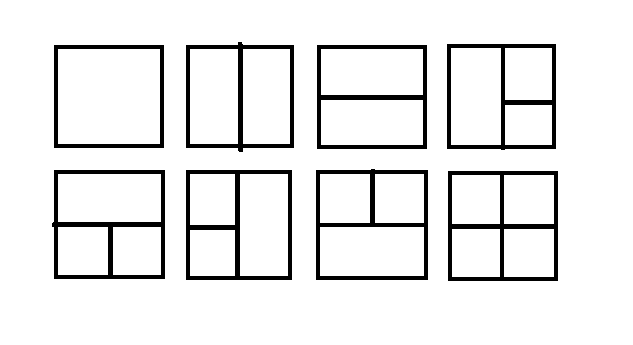
\includegraphics[width=0.65\textwidth]{Block_types} % Include the image placeholder.png
\caption{Diagrams of all valid block layouts.}
\end{center}
\end{figure}

After a city block has been assigned a sub-block combination each sub-block then gets assigned a building type. In my city, buildings consist of three types: towers, businesses, and residences. Each type has unique geometry and different parameters with regards to maximum height. In addition to those differences, each building type has a probability of appearing that varies according to which 'zone' the city block resides in. The centre of the city block grid is zone 0, while all of the blocks surrounding zone 0 belong to zone 1, and the blocks outside of that ring of blocks belong to zone 2 and so on. I use the cosine function to generate thresholds for each zone, then I randomly generate a number between 0 and 1 and compare that against the threshold value of the zone and, if necessary, the zone before. These thresholds have the affect of splitting the range 0-1 and, depending on which portion of that range the randomly generated number falls into, a number corresponding to a building type is returned. The overall affect of this system is that as you get further away from the centre towers become less common and residential buildings become more common. Businesses are most likely to spawn in the midrange zones. For more details see the functions rbt\_non\_uniform and calc\_zone\_thresh. \par

With the building type selected all that remains is for a specific model to be selected. There are three separate functions containing the generation code for each type of building, within each one the first step is to determine the size of the sub-block. For each size of sub-block there are different models because, of course, the size of the sub-block limits the maximum size of the building. Once the size of the sub-block has been determined a random number is generated in order to determine which model will be generated as there are several different models for each sub-block size. The exception to this process is residential buildings as they have only one model and sometimes are not generated in order to give the city a more realistic, sparse aesthetic. The buildings are all constructed from primitive cubes which are then scaled and translated and combined to make more complex geometry. After that a material and texture is applied, making sure to apply different colours to differnt parts of the buildings.

Building generation is complete when every sub-block of every city block has been processed. Following this, a plane is constructed to fit underneath the city blocks and then textured to look somewhat like asphalt. Finally, lighting and cameras are set up.


\section{Results}

With eight different block layouts, and over 12 different building models (some are scaled versions of larger buildings) my script can generate a fair variety of different cities. In addition to this, building height varies according to random number generation and predefined parameters making each permutation look more distinct. The cosine thresholding and zoning system appears to generate a nice distribution of building types that looks like something you might expect to see in a real city. 

\begin{figure}[H]
\begin{center}
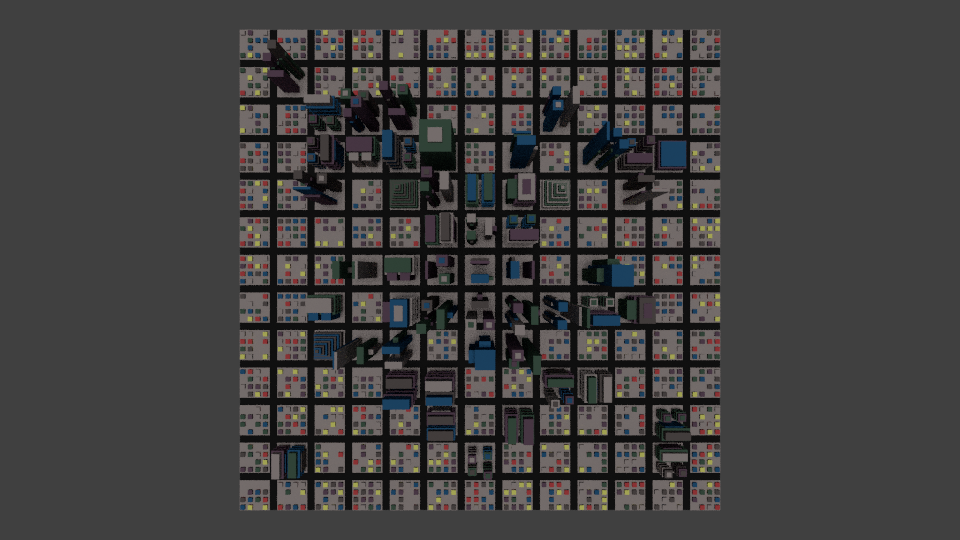
\includegraphics[width=0.65\textwidth]{render13_cycles0} % Include the image placeholder.png
\caption{Top-down view. 13x13 Grid. Cycles Rendering.}
\end{center}
\end{figure}

\begin{figure}[H]
\begin{center}
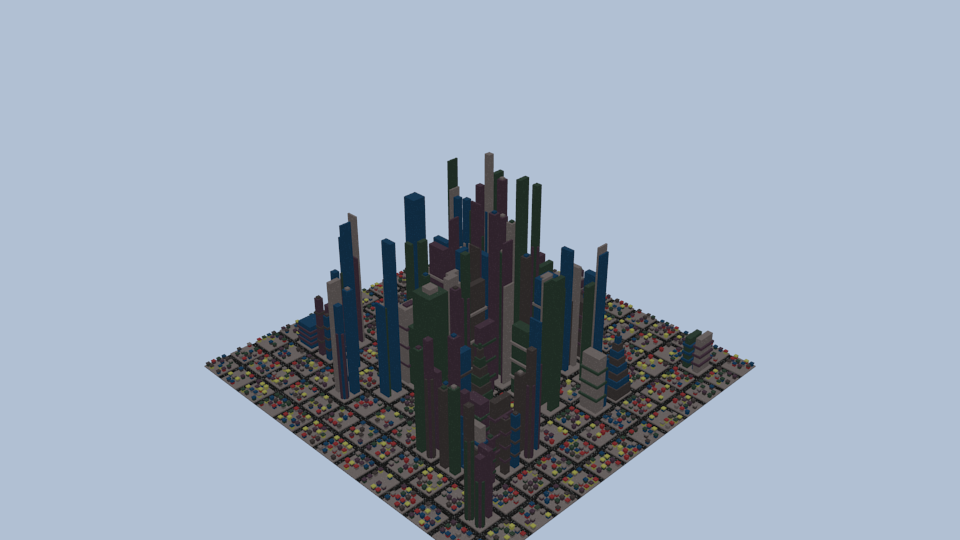
\includegraphics[width=0.65\textwidth]{render1} % Include the image placeholder.png
\caption{Angled view. 13x13 Grid. Blender Rendering.}
\end{center}

\end{figure}
\begin{figure}[H]
\begin{center}
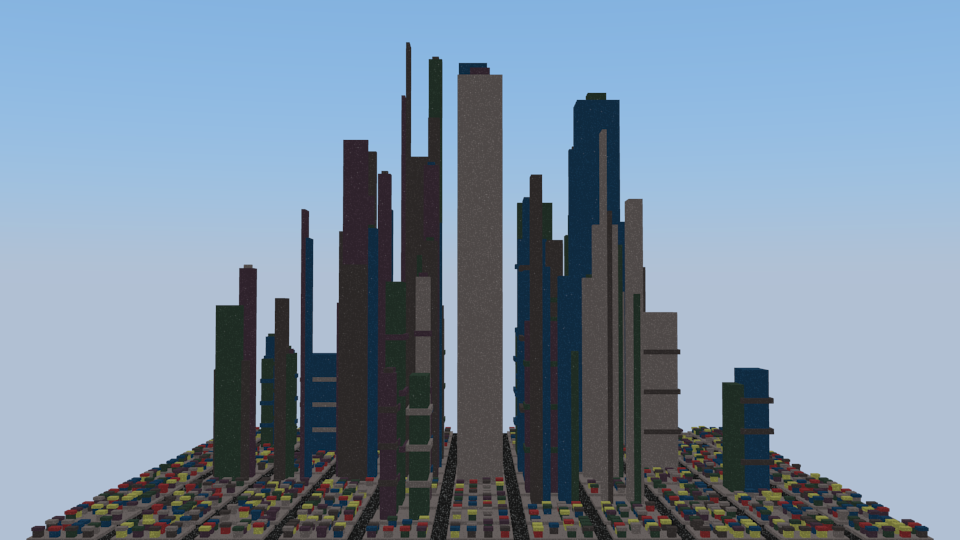
\includegraphics[width=0.65\textwidth]{render0-11} % Include the image placeholder.png
\caption{Side-on view. 11x11 Grid. Blender Rendering.}
\end{center}
\end{figure}

\section{Discussion and Future Work}

Because of the time I wasted, as discussed in the planning section, there are a number of elements of the final product that I feel didn't get enough attention. Primary among these elements are the materials and texturing. I attempted to apply an image texture to some of the buildings but couldn't figure out how to do so convincingly in a timely manner. Because of this, the texture I used on the buildings was a simple noise texture that served to make the buildings look somewhat less plastic. Given more time I would have liked to have the buildings look more real. 

Another aspect is the lighting and, in relation to this, the choice of rendering engine. As you can see in the three figures above, two of these are rendered with the Blender rendering engine and the other is with the Cycles rendering engine. In my opinion the Cycles rendering is far more visually impressive than the Blender rendering. However I couldn't configure the lighting in the Cycles engine, again due to time constraints. 

Lastly I feel as though my code is far more bloated than it needed to be. In each of the functions used to generate buildings there is a lot of repeated code with small changes each time. I simply didn't have the time to think of a more intelligent way to structure all of the various cases into a few methods. 

Despite all of that, I am happy with how the script and subsequent models turned out. 


\end{document}